\section{Verformungen}



	\begin{minipage}{0.5\linewidth}

		\subsection{Verformung am Zugstab}
		
			
	\textbf{Gerissen: (N > N$_r$) }
	
	\begin{tabular}{lp{0.3\linewidth}}
		
		Dehnung (Grenzfall im Riss):		& $ \varepsilon^{II} =  \frac{N}{A_s \cdot n \cdot E_c} $ \\
		
		Verformung (obere Schranke):		& $ \Delta l = l_0 \varepsilon^{II} $ \\
		
		Mitwirkung zwischen den Rissen	& \\
		
		Kriechen:						& kein Einfluss, da keine Druckbeanspruchung im Beton \\
		
	\end{tabular}
	
\end{minipage}
\begin{minipage}{0.5\linewidth}
		
		
		\textbf{Ungerissen: (N < N$_r$) }
		
		\begin{tabular}{ll}
			Dehnung:		& $ \varepsilon = \frac{N}{A_i \cdot E_c} $ \\
			
			Verformung:		& $ \Delta l = l_0 \varepsilon $ \\
			
			Schwinden:		& Verformung \\
			
		\end{tabular}
				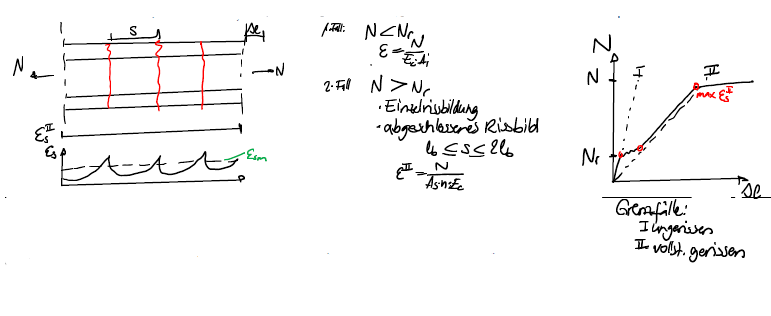
\includegraphics[width=\linewidth]{images/Verformung1Zustand.PNG}
	\end{minipage}



\textcolor{red}{Vorlesung 07, Folie 5 (Kriechen. Schwinden, Tension Stiffening, Durchbiegung), SIA 260 Durchbiegung berechnen}